\documentclass{article}

% if you need to pass options to natbib, use, e.g.:
%     \PassOptionsToPackage{numbers, compress}{natbib}
% before loading neurips_2018
\usepackage{marvosym,graphicx,subfloat,subfig,tikz}

\usepackage{graphicx} 
\usepackage[numbers]{natbib}


% ready for submission
%\usepackage{neurips}

% to compile a preprint version, e.g., for submission to arXiv, add add the
% [preprint] option:
%\usepackage[preprint]{neurips}
\usepackage{natbib}
% to compile a camera-ready version, add the [final] option, e.g.:
\usepackage[final]{neurips}
\usepackage{lipsum}
% to avoid loading the natbib package, add option nonatbib:
%     \usepackage[nonatbib]{neurips_2018}
\usepackage{rotating}

\usepackage[utf8]{inputenc} % allow utf-8 input
\usepackage[T1]{fontenc}    % use 8-bit T1 fonts
\usepackage{hyperref}       % hyperlinks
\usepackage{url}            % simple URL typesetting
\usepackage{booktabs}       % professional-quality tables
\usepackage{amsfonts}       % blackboard math symbols
\usepackage{nicefrac}       % compact symbols for 1/2, etc.
\usepackage{microtype}      % microtypography

\title{Predominant Musical Instrument Classification based on Spectral Features}

% The \author macro works with any number of authors. There are two commands
% used to separate the names and addresses of multiple authors: \And and \AND.
%
% Using \And between authors leaves it to LaTeX to determine where to break the
% lines. Using \AND forces a line break at that point. So, if LaTeX puts 3 of 4
% authors names on the first line, and the last on the second line, try using
% \AND instead of \And before the third author name.

\author{%
  No name given\\
  Indian Statistical Institute\\
  Kolkata, WB 700 108}
  % examples of more authors
  % \And
  % Coauthor \\
  % Affiliation \\
  % Address \\
  % \texttt{email} \\
  % \AND
  % Coauthor \\
  % Affiliation \\
  % Address \\
  % \texttt{email} \\
  % \And
  % Coauthor \\
  % Affiliation \\
  % Address \\
  % \texttt{email} \\
  % \And
  % Coauthor \\
  % Affiliation \\
  % Address \\
  % \texttt{email} \\

\begin{document}
% \nipsfinalcopy is no longer used

\maketitle

\begin{abstract}
  This work aims to examines one of the corner stone problem of Musical Instrument Retrieval in particular instrument classification. We have presented a very concise summary of past work in this domain. We have included most of  code (jupyter notebook) for easy reproducibility.
\end{abstract}


%\section{Submission of papers to NeurIPS 2018}

\section{Introduction}
\lipsum[6]
\subsection{Motivation of our work}

\subsection{Related Works}
\section{Results \& Discussion}



\bibliographystyle{plainnat}


\subsection{Our Contribution}

In solving any classification problem of audio and video file the most important thing is to choose how to extract features from given audio/video files. While dealing with our audio dataset we found that despite having  the same  notes of sound, spectrogram differs based on which instrument is playing that note. As an illustration we recorded the same note with 4 different instruments and generated the corresponding spectrograms in Figure \ref{fig:instr}. It is evident that we can use this property of spectrogram to predict instrument used while playing particular sound excerpt. 


According to \citet{Eronen2000} Timbre, perceptually, is the `colour' of a sound. Experiments have sought to construct a low-dimensional space to accommodate similarity ratings. Efforts are then made to interpret these ratings acoustically or perceptually.
The two principal dimensions here are spectral centroid and rise time. Spectral centroid corresponds to the perceived brightness of sound. Rise time measures the time difference between the start and the moment of highest amplitude.

\citet{deng2008study} have shown instruments usually have some unique properties that can be described by their 
harmonic spectra and their temporal and spectral envelopes. They have shown only first few coefficients are enough for proper classification.

To do the spectral analysis MFCC is best choice. According to Wikipedia\cite{wiki:00} ``the mel-frequency cepstrum (MFC) is a representation of the short-term power spectrum of a sound, based on a linear cosine transform of a log power spectrum on a nonlinear mel scale of frequency''. Mel is a number that links to a pitch, which is analogous to how a frequency is described by a pitch. The basic flow of calculating the MFC Coefficients is outlined below


\tikzset{every picture/.style={line width=0.65pt}} %set default line width to 0.75pt        
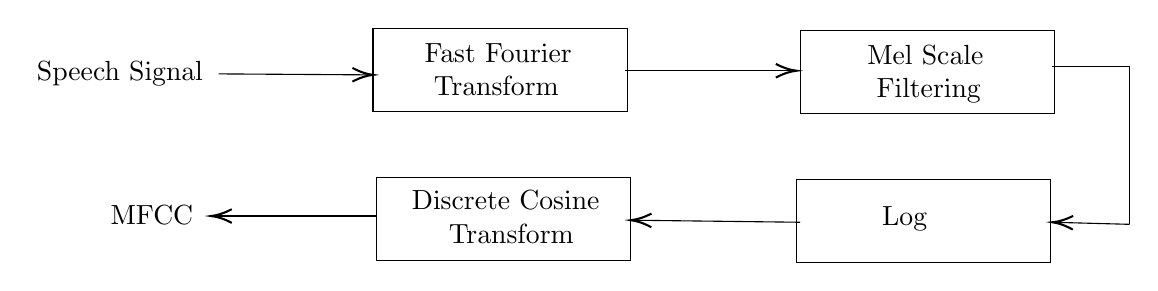
\begin{tikzpicture}[x=0.68pt,y=0.75pt,yscale=-1,xscale=1]
%uncomment if require: \path (0,141.484375); %set diagram left start at 0, and has height of 141.484375

%Shape: Rectangle [id:dp7748808264891436] 
\draw   (200,11) -- (335,11) -- (335,51) -- (200,51) -- cycle ;
%Shape: Rectangle [id:dp5514439247330727] 
\draw   (427,12) -- (562,12) -- (562,52) -- (427,52) -- cycle ;
%Shape: Rectangle [id:dp15640091794986954] 
\draw   (425,84) -- (560,84) -- (560,124) -- (425,124) -- cycle ;
%Shape: Rectangle [id:dp8469318664749113] 
\draw   (202,83) -- (337,83) -- (337,123) -- (202,123) -- cycle ;
%Straight Lines [id:da382056424047289] 
\draw    (118,33) -- (198,33.47) ;
\draw [shift={(200,33.48)}, rotate = 180.34] [color={rgb, 255:red, 0; green, 0; blue, 0 }  ][line width=0.75]    (10.93,-3.29) .. controls (6.95,-1.4) and (3.31,-0.3) .. (0,0) .. controls (3.31,0.3) and (6.95,1.4) .. (10.93,3.29)   ;

%Straight Lines [id:da6128304587056241] 
\draw    (334,31.48) -- (423,31.48) ;
\draw [shift={(425,31.48)}, rotate = 180] [color={rgb, 255:red, 0; green, 0; blue, 0 }  ][line width=0.75]    (10.93,-3.29) .. controls (6.95,-1.4) and (3.31,-0.3) .. (0,0) .. controls (3.31,0.3) and (6.95,1.4) .. (10.93,3.29)   ;

%Straight Lines [id:da3628527645252546] 
\draw    (427,104.48) -- (339,103.51) ;
\draw [shift={(337,103.48)}, rotate = 360.64] [color={rgb, 255:red, 0; green, 0; blue, 0 }  ][line width=0.75]    (10.93,-3.29) .. controls (6.95,-1.4) and (3.31,-0.3) .. (0,0) .. controls (3.31,0.3) and (6.95,1.4) .. (10.93,3.29)   ;

%Straight Lines [id:da685339938155058] 
\draw    (202,101.48) -- (116,101.48) ;
\draw [shift={(114,101.48)}, rotate = 360] [color={rgb, 255:red, 0; green, 0; blue, 0 }  ][line width=0.75]    (10.93,-3.29) .. controls (6.95,-1.4) and (3.31,-0.3) .. (0,0) .. controls (3.31,0.3) and (6.95,1.4) .. (10.93,3.29)   ;

%Straight Lines [id:da5358151917118492] 
\draw    (561,29.48) -- (602,29.48) ;


%Straight Lines [id:da7191560755449415] 
\draw    (602,29.48) -- (602,105.48) ;


%Straight Lines [id:da8210553796100066] 
\draw    (602,105.48) -- (563,104.53) ;
\draw [shift={(561,104.48)}, rotate = 361.4] [color={rgb, 255:red, 0; green, 0; blue, 0 }  ][line width=0.75]    (10.93,-3.29) .. controls (6.95,-1.4) and (3.31,-0.3) .. (0,0) .. controls (3.31,0.3) and (6.95,1.4) .. (10.93,3.29)   ;


% Text Node
\draw (65.5,33) node  [align=left] {Speech Signal};
% Text Node
\draw (266.5,31) node  [align=left] {Fast Fourier \\ \ Transform};
% Text Node
\draw (493.5,33) node  [align=left] {Mel Scale \\ \ Filtering};
% Text Node
\draw (482.5,103) node  [align=left] {Log};
% Text Node
\draw (270.5,102) node  [align=left] {Discrete Cosine \\ \ \ \ \ Transform};
% Text Node
\draw (82.5,101) node  [align=left] {MFCC};


\end{tikzpicture}

The mathematical formula for frequency-to-mel transform is $$m=2595\,\log_{10}\left(1+\frac f{700}\right).$$
\begin{figure}[!htb]
	\centering
	\subfloat[EDM ]{\label{fig:edm}\includegraphics[width=70mm]{EDM.png}}
	\subfloat[Guitar (Accoustic) ]{\label{fig:gac}\includegraphics[width=70mm]{Guitar.png}}
	\\
	\subfloat[Key Board ]{\label{fig:key}\includegraphics[width=70mm]{keyboard.png}}
	\subfloat[Organ ]{\label{fig:org}\includegraphics[width=70mm]{Organ.png}}
	\caption{Same note (audio) played in various instruments and their spectograms}
	\label{fig:instr}
\end{figure}


MFCCs are obtained by transforming frequency (hertz) scale to mel scale. Typically, MFCC coefficients are numbered from the $0$th to 20th order and the first 13 coefficients are more than enough to do any kind of audio classification task.


\subsection{Dataset}
 We used IRMAS(Instrument recognition in Musical Audio Signals)\cite{bosch2012comparison} dataset in our study as this is a  polyphonic dataset so we can use it train a robust classifier.  The data consists of \texttt{.wav} files of 3 seconds duration of many instruments, about eleven. We have chosen six of these instruments (viz. flute, piano, trumpet, guitar, voice and organ) for recognition. Our data has 3846 samples of music running into about three hours, giving sufficient data for training and testing purposes as well. In addition, the data consists of multiple genres including country folk, classical, pop-rock and latin soul. Inclusion of these multiple genres could lead to better training. 
The dataset has been downloaded from  \url{https://www.upf.edu/web/mtg/irmas}. Number of audio samples per instrument class is reproduced in table \ref{tab:ic}.

\begin{table}[h!]
	\begin{tabular}{@{}lcc@{}}
		\textbf{Instrument} & \textbf{Number of Samples} & \multicolumn{1}{l}{\textbf{Clip Length (in sec)}}           \\\midrule
		Flute               & 451                        & 1353                                                        \\
		Piano               & 721                        & 2163                                                        \\
		Trumpet             & 577                        & 1731                                                        \\
		Guitar              & 637                        & 1911                                                        \\
		Voice               & 778                        & 2334                                                        \\
		Organ               & 682                        & 2046                                                        \\
		\textbf{Total}               & 3846                       & 11538 (3 hr 12 min) 
	\end{tabular}
\vspace{0.1in}
\caption{Instrument Samples and Clip Length}
	\label{tab:ic}
\end{table}



\section{Methodology \& Our Approach}

\subsection{Feature Extraction}
\citet{deng2008study} have shown that for achieving more accurate classification of musical instruments, it is essential to extract more complicated features in our analysis, apart from MFCC. Hence, we considered other features like Zero-crossing rate, Spectral centroid, Spectral bandwidth and Spectral roll-off during our feature extraction via Librosa. Zero Crossing rate indicates the rate at which the signal crosses zero. Spectral Centroid is a measure to indicate the center of mass of the spectrum being located, featuring the impression of brightness characteristic given a sound sample. Spectral bandwidth gives the weighted average of the frequency signal by its spectrum. Spectral roll-off features the frequency under which a certain proportion of the overall spectral energy belongs to.


To extract features from audio files we needed to use any library. We had two options -- Librosa\cite{mcfee2015librosa} and Essentia\cite{esen}. We tried with both of libraries. 


Essentia is  an open-source C++ based distribution package available under Python environment for audio-based musical information retrieval. This library computes spectral energy associated with mel bands and their MFCCs given an audio sample.

Windowing procedure is also implemented in Essentia for analyzing the frequency content of an audio spectrum by creating a short sound segments of a few milli-seconds for a relatively longer signal. By default, we used Hann window, a smoothing window typically characterized with not only having good frequency resolution but also reduced spectral leakage.

The audio spectrum is analyzed by extracting MFCCs based on the default inputs of hopSize (determines the hop length between frames) and frame size given. The default parameters for sampling rate is 44.1 kHz, the hop length (HopSize) 512 and frame size as 1024 in Essentia. This features thus extracted from manifold segments of a sample signal are aggregated with their mean and used as the features for each sample labeled with their instrument class.

On the other hand, Librosa --- the Python package used for music and audio data analysis. The only distinction  is the rate of audio sampling, where it is resampled at 22.05 kHz during load time.

Among both the libraries we prefered Librosa as it fetched more accuracy as well as being an older software package there was a lot of community support from various online forums. 

\subsection{Classifier Training}

We have applied various machine learning techniques to perform  classification of instruments.

MFCC features were extracted using librosa/essentia. We extracted first 13 MFCC features. We got 2048 $\times$ 13 matrix feature for a particular audio clip. We took mean of all the columns to get condensed feature providing us with 1 $\times$ 13 feature vector. As mentioned above 5 other features were also appended in that feature vector. Using the labelencoder function of scikit learn we labeled each vector with the instrument class it belonged to.

\paragraph{Supervised Classification Techniques}
We used different supervised classification techniques to identify the predominant musical instrument from the audio file. We used scikit learn\cite{scikit} to train our classifer in a jupyter based python3 notebook. Initially we started with logistic regression and decision tree classifier. Classification trees are usually prone to overfitting, So it did not perform well on the test data. We also fit some bagging and boosting techniques on the mfcc and spectral features. We tried random forest to control the overfitting and with some parameter tuning, it provided us with the better classification. We also tried XGBoost on the same set of features and after some parameter tuning gradient boosting classified the instruments with an accuracy of around 0.7. 


Support vector machine (SVM) was also used to fit the extracted features. It outperformed the other traditional classification techniques mentioned above. We used radial basis function kernel for this non linear classification. We also performed some parameter tuning for penalty parameter C and kernel coefficient gamma which improved the overall accuracy on test data.


We also designed a simple neural network to perform this classification. We used three layers with 30, 15 and 6 neurons on these layers respectively. We applied relu activation function on the first two layers and sigmoid on the last layer of the network. Neural network also performed better than most of the traditional techniques mentioned above.


In terms of accuracy bagging and boosting models such as random forest and XGboost performed better than traditional models such as classification trees and logistic regression. Finally SVM turned out to be a more accurate classifier than other techniques mentioned above.

\subsection{Evaluation Criteria}

The following evaluation metrics were used to judge the performance of the model

\begin{itemize}
	\item The precision is the ratio $\frac{tp}{(tp + fp)}$ where $tp$ is the number of true positives and $fp$ the number of false positives. The precision is intuitively the ability of the classifier not to label as positive a sample that is negative. Precision for various models are shown in a boxplot format see Fig: \ref{fig:precision}. 
	
	\item The recall is the ratio  $\frac{tp}{(tp + fn)}$ where $tp$ is the number of true positives and $fn$ the number of false negatives. The recall is intuitively the ability of the classifier to find all the positive samples. Fig: \ref{fig:recall} shows illustrative visulization for various supervised model. 
	
	\item The F1 score can be interpreted as a weighted average of the precision and recall. $$F1 = \frac{2 * (\rm{precision} * \rm{recall})}{ (\rm{precision} + \rm{recall})}$$
	
	\item Confusion Matrix is a technique to evaluate performance of a supervised classification. Calculating a confusion matrix gives a better idea of what our classification model is getting right and what types of errors it is making. Confusion Matrix for various models is shown in Fig: \ref{figur}
	
		
	% Please add the following required packages to your document preamble:
	% \usepackage{booktabs}
	\begin{center}
		\begin{table}[h!]
			\begin{tabular}{@{}l|lll|lll|lll@{}}
				\toprule
				& \multicolumn{3}{c}{\textbf{Logistic Regession}}                        & \multicolumn{3}{c}{\textbf{Decision Tree}}                             & \multicolumn{3}{c}{\textbf{LGBM}}                                      \\ \midrule
				Instrument & \multicolumn{1}{c}{P} & \multicolumn{1}{c}{R} & \multicolumn{1}{c}{F1} & \multicolumn{1}{c}{P} & \multicolumn{1}{c}{R} & \multicolumn{1}{c}{F1} & \multicolumn{1}{c}{P} & \multicolumn{1}{c}{R} & \multicolumn{1}{c}{F1}\\ 
				Flute      & 0.58                  & 0.39                  & 0.47                   & 0.43                  & 0.44                  & 0.43                   & 0.66                  & 0.59                  & 0.62                   \\
				Piano      & 0.55                  & 0.59                  & 0.57                   & 0.53                  & 0.54                  & 0.53                   & 0.69                  & 0.73                  & 0.71                   \\
				Trumpet    & 0.44                  & 0.53                  & 0.48                   & 0.50                  & 0.46                  & 0.48                   & 0.59                  & 0.67                  & 0.63                   \\
				Guitar     & 0.63                  & 0.57                  & 0.60                   & 0.60                  & 0.57                  & 0.58                   & 0.73                  & 0.68                  & 0.71                   \\
				Voice      & 0.58                  & 0.48                  & 0.52                   & 0.52                  & 0.50                  & 0.51                   & 0.72                  & 0.54                  & 0.62                   \\
				Organ      & 0.51                  & 0.61                  & 0.56                   & 0.50                  & 0.55                  & 0.52                   & 0.63                  & 0.74                  & 0.68                   \\ 
			\end{tabular}
			
			
			\begin{tabular}{@{}l|lll|lll|lll@{}}
				\toprule
				& \multicolumn{3}{c}{\textbf{XG Boost}}                                  & \multicolumn{3}{c}{\textbf{RF}}                                        & \multicolumn{3}{c}{\textbf{SVM}}                                       \\ \midrule
				Instrument & \multicolumn{1}{c}{P} & \multicolumn{1}{c}{R} & \multicolumn{1}{c}{F1} & \multicolumn{1}{c}{P} & \multicolumn{1}{c}{R} & \multicolumn{1}{c}{F1} & \multicolumn{1}{c}{P} & \multicolumn{1}{c}{R} & \multicolumn{1}{c}{F1} \\
				Flute      & 0.66                  & 0.59                  & 0.62                   & 0.72                  & 0.48                  & 0.58                   & 0.63                  & 0.63                  & 0.63                   \\
				Piano      & 0.72                  & 0.71                  & 0.71                   & 0.72                  & 0.75                  & 0.74                   & 0.79                  & 0.84                  & 0.81                   \\
				Trumpet    & 0.58                  & 0.69                  & 0.63                   & 0.61                  & 0.72                  & 0.66                   & 0.78                  & 0.77                  & 0.78                   \\
				Guitar     & 0.71                  & 0.72                  & 0.71                   & 0.73                  & 0.72                  & 0.72                   & 0.77                  & 0.76                  & 0.77                   \\
				Voice      & 0.75                  & 0.53                  & 0.62                   & 0.74                  & 0.54                  & 0.62                   & 0.78                  & 0.67                  & 0.72                   \\
				Organ      & 0.65                  & 0.74                  & 0.69                   & 0.63                  & 0.80                  & 0.70                   & 0.79                  & 0.85                  & 0.82                   \\ \bottomrule
			\end{tabular}
			\vspace{0.1 in }
			\caption{Precision, Recall \& F1 Score for  various Supervised Models}
		\end{table}
		
	\end{center}
	
\end{itemize}
\begin{figure}[htp]
	\centering
	\subfloat[Logistic Regression ]{\label{figur:1}\includegraphics[width=80mm]{LogisticRegression.png}}
	\subfloat[Decsion Tree ]{\label{figur:2}\includegraphics[width=80mm]{DecisionTree.png}}
	\\
	\subfloat[Light GBM ]{\label{figur:3}\includegraphics[width=80mm]{LGBM.png}}
	\subfloat[XG Boost ]{\label{figur:4}\includegraphics[width=80mm]{xgboost.png}}
	\\
	\subfloat[Random Forest ]{\label{figur:5}\includegraphics[width=80mm]{RandomForest.png}}
	\subfloat[SVM  ]{\label{figur:6}\includegraphics[width=80mm]{SVM.png}}
	\caption{Confusion Matrix for various supervised Algorithms}
		\label{figur}
	
\end{figure}




%%pre recall main boxplot
\begin{figure}
	\centering
	
		\subfloat[Precision ]{\label{fig:precision}\includegraphics[width=80mm]{precision.pdf}}
	\subfloat[Recall ]{\label{fig:recall}\includegraphics[width=80mm]{recall.pdf}}
	\\
	\subfloat[F1 Score ]{\label{fig:f1}\includegraphics[width=80mm]{f1.pdf}}
	\subfloat[Accuracy ]{\label{fig:acc}\includegraphics[width=80mm]{acc.pdf}}
	\caption{Evaluation Metric for Various Supervised Algorithms}
\end{figure}

%%instru class
\begin{figure}
	\centering
	\includegraphics[width=0.8\linewidth]{instr-f1}
	\caption{Instrument wise classification}
	\label{fig:instrument-f1}
\end{figure}







\subsubsection*{Acknowledgments}

Use unnumbered third level headings for the acknowledgments. All acknowledgments
go at the end of the paper. Do not include acknowledgments in the anonymized
submission, only in the final paper. 
 \bibliographystyle{unsrt}. \bibliography{bibo}


\end{document}
